\documentclass{standalone}
\usepackage{tikz}
\usetikzlibrary{bbox}
\usetikzlibrary{calc}
\usetikzlibrary{arrows.meta,decorations.pathmorphing,backgrounds,positioning,fit,petri}

\def\centerarc[#1](#2)(#3:#4:#5)% Syntax: [draw options] (center) (initial angle:final angle:radius)
    { \draw[#1] ($(#2)+({#5*cos(#3)},{#5*sin(#3)})$) arc (#3:#4:#5); }

\definecolor{mygreen}{RGB}{120,220,160}
\definecolor{mydarkgreen}{RGB}{60,120,60}
\definecolor{myverydarkgreen}{RGB}{20,60,20}
\definecolor{myblue}{RGB}{10,140,220}
\definecolor{mydarkblue}{RGB}{60,60,120}

\begin{document}
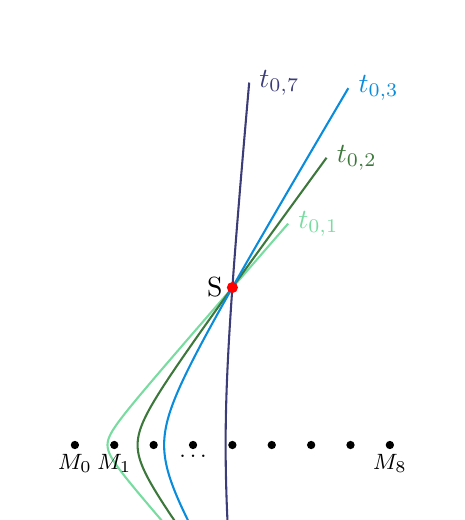
\begin{tikzpicture}
    [wave/.style={white!50!red,thick}]

    \def\tmax{3.4}
    \def\N{100}
    \def\a{0.164}
    \def\b{0.188}
    \draw[color=mygreen,line width=0.75,samples=\N,variable=\t,domain=-\tmax:\tmax] % left
        plot({\a*cosh(\t) -1.75},{\b*sinh(\t) -2}) node[right] {$t_{0,1}$};
    \def\tmax{2.9}
    \def\a{0.296}
    \def\b{0.403}
    \draw[color=mydarkgreen,line width=0.75,samples=\N,variable=\t,domain=-\tmax:\tmax] % left
        plot({\a*cosh(\t) -1.5},{\b*sinh(\t) -2}) node[right] {$t_{0,2}$};
    \def\tmax{2.65}
    \def\a{0.383}
    \def\b{0.644}
    \draw[color=myblue,line width=0.75,samples=\N,variable=\t,domain=-\tmax:\tmax] % left
        plot({\a*cosh(\t) -1.25},{\b*sinh(\t) -2}) node[right] {$t_{0,3}$};
    \def\tmax{1.7}
    \def\a{0.164}
    \def\b{1.742}
    \draw[color=mydarkblue,line width=0.75,samples=\N,variable=\t,domain=-\tmax:\tmax] % left
        plot({\a*cosh(\t) -0.25},{\b*sinh(\t) -2}) node[right] {$t_{0,7}$};

    % \def\a{-0.296}
    % \def\b{0.403}
    % \draw[color=mydarkblue,line width=0.5,samples=\N,variable=\t,domain=-\tmax:\tmax] % left
    %     plot({\a*cosh(\t) +1.5},{\b*sinh(\t) -2});

    \coordinate[label=left:{S}] (origin) at (0,0);
    \fill[red] (origin) circle (2pt);

    % \centerarc[wave](origin)(0:360:0.5)
    % \centerarc[wave](origin)(0:360:1)
    % \centerarc[wave](origin)(0:360:1.5)
    % \centerarc[wave](origin)(0:360:2.0)
    % \centerarc[wave](origin)(0:360:2.5)
    % \centerarc[wave](origin)(0:360:3)
    % \centerarc[wave](origin)(0:360:3.5)
    % \centerarc[wave](origin)(0:360:4)

%    \draw[scale=2,domain=-1.5:1.5,smooth,variable=\t] 
%                plot ({0.164/2*sec(\t r)-1.75/2},{0.188/2*tan(\t r)-2/2});

    

    \fill (-2,-2) circle (1.5pt) node[below] {\footnotesize$M_0$};
    \fill (-1.5,-2) circle (1.5pt) node[below] {\footnotesize$M_1$};
    \fill (-1,-2) circle (1.5pt);
    \fill (-0.5,-2) circle (1.5pt) node[below] {\footnotesize $\dots$};
    \fill (-0.0,-2) circle (1.5pt);
    \fill (0.5,-2) circle (1.5pt);
    \fill (1,-2) circle (1.5pt);
    \fill (1.5,-2) circle (1.5pt);
    \fill (2.0,-2) circle (1.5pt) node[below] {\footnotesize$M_8$};

    
    % \node[label={Array}] at (0.45,-2) {};

    % \draw [<->] (0,-1.9) -- (0,0) node[midway,left]{$R \leq \phi$};
    % \draw [<->] (-2,-2.1) -- (2, -2.1) node[midway,below]{$\phi$};

    \pgfresetboundingbox
    \useasboundingbox(-2.6,-2.6)rectangle(2.6,3.3);
\end{tikzpicture}
\end{document}